\chapter{
MCMC for Spatial Capture-Recapture
}
\markboth{MCMC}{}
\label{chapt.mcmc}

%%% NOTES
%%% Andy's working through this doing format edits mostly and math
%%% stuff , but not in order
%%% anytime you see a XXX or XYZ that is a marker to change some
%%% hard-wired reference to a float

\vspace{.3in}

\section{Introduction}
In this chapter we will dive a little deeper into Markov chain Monte
Carlo (MCMC) sampling. We will construct custom MCMC samplers in {\bf R},
starting with easy-to-code GLMs and GLMMs and moving on to simple CR and SCR
models. Finally, we will illustrate some alternative
ready-to-use software packages for MCMC sampling. We will NOT provide
exhaustive background information on the theory and justification of
MCMC sampling – there are entire books dedicated to that subject and
we refer you to \citet{robert_casella:2004} and
\citet{robert_casella:2010}. Rather we aim to provide you with enough
background and technical know-how to start building your own MCMC
samplers for SCR models in {\bf R}. You will find that quite a few topics that come up 
in this chapter have already been covered in previous chapters, particularly the introduction
into Byesian analysis in Chapt. \ref{chapt.glms}. To keep you from having to leaf back and forth
we will in some places briefly review aspects of Bayesian analysis, but we try to focus on the more 
technical issues of building MCMC samplers. 



\subsection{Why build your own MCMC algorithm?}

The standard program we have used so far to run MCMC analyses is
WinBUGS \citep{gilks_etal:1994}. The wonderful thing about WinBUGS is
that it will automatically use the most appropriate and efficient form
of MCMC sampling for the model specified by the user.

The fact that we have such a Swiss Army knife type of MCMC machine
begs the question: Why would anyone want to build their own MCMC
algorithm? For one, there are a limited number of distributions and
functions implemented in WinBUGS. While OpenBUGS provides more
options, some more complex models may be impossible to build within
these programs. A very simple example from spatial capture-recapture
that can give you a headache in WinBUGS is when your state-space is an
irregular-shaped polygon, rather than an ideal rectangle that can be
characterized by four pairs of coordinates. It is easy to restrict
activity centers to any arbitrary polygon in R using an ESRI shapefile
(and we will show you an example in a little bit), but you cannot use
a shape file in a BUGS model.

Sometimes implementing an MCMC algorithm in R may be faster than in
WinBUGS - especially if you want to run simulation studies where you
have hundreds or more simulated data sets, several years' worth of
data or other large models, this can be a big advantage.

Finally, building your own MCMC algorithm is a great exercise to understand how MCMC sampling works. So while using the BUGS language requires you to understand the structure of your model, building an MCMC algorithm requires you to think about the relationship between your data, priors and posteriors, and how these can be efficiently analyzed and characterized. Not to mention that, if you are an R junkie, it can actually be fun.
However, if you don't think you will ever sit down and write your own
MCMC sampler, consider skipping this chapter - apart from coding it
will not cover anything SCR-related that is not covered by other, more
model-oriented chapters as well.


\section{MCMC and posterior distributions}

As mentioned in Chapter 2, MCMC is a class of simulation methods for
drawing (correlated) random numbers from a target distribution, which
in Bayesian inference is the posterior distribution.
As a reminder, the posterior distribution is a probability
distribution for an unknown parameter, say $\theta$, given a set of
observed data and its prior probability distribution (the probability
distribution we assign to a parameter before we observe data).  The
great benefit of computing the posterior distribution of $\theta$ is
that it can be used to make probability statements about $\theta$,
such as the probability that $\theta$ is equal to some value, or the
probability that $\theta$ falls within some range of values. 
The posterior distribution summarizes all we know about a parameter
and thus, is the central object of interest in Bayesian
analysis. Unfortunately, in many if not most practical applications,
it is nearly impossible to directly compute the posterior. Recall
Bayes’ theorem:
\begin{equation}
p(\theta|y) = p(y|\theta) * p(\theta) / p(y),
\label{mcmc.eq.bayes}
\end{equation}
where $\theta$ is the parameter of interest, $y$ is the observed data,
$p(\theta|y)$ is the posterior, $p(y|\theta)$ the likelihood of the
data conditional on $\theta$, $p(\theta)$ the prior probability of
$\theta$, and, finally, $p(y)$ is the marginal probability of the
data, which can also be written as
\[
p(y) = \int p(y|\theta) * p(\theta) d\theta
\]

This marginal probability is a normalizing constant that ensures that
the posterior integrates to 1. This
integral is often hard or impossible to evaluate, unless you are
dealing with a really simple model.  For example, consider that you
have a Normal model, with a set of n observations, $y$ that come from a
Normal distribution:
\[
 y \sim \mbox{Normal}(\mu, \sigma),
\]
where $\sigma$ is known and our objective is to obtain an estimate of
$\mu$ using Bayesian statistics. To fully specify the model in a Bayesian
framework, we first have to define a prior distribution for $\mu$. Recall
from Chapter 2 that for certain data models, certain priors lead to
conjugacy – i.e. if you choose the right prior for your parameter,
your posterior distribution will be of a known parametric form. The
conjugate prior for the mean of a normal model is also a Normal
distribution:
\[
\mu \sim \mbox{Normal}(\mu_0, \sigma_{0}^{2})
\]
If $\mu_{0}$ and $\sigma_{0}^{2}$ are fixed, the posterior for $\mu$ has the following form (for the algebraic proof, see XXX):
\begin{equation}
\mu|y \sim \mbox{Normal}(\mu_{n}, \sigma_{n}^{2})
\label{mcmc.eq.mu-posterior}
\end{equation}
where
\[
\mu_{n} = \frac{ \sigma^{2}}  {\sigma^{2}   +n* \sigma_{0}^{2}}*  \mu_0 +      \frac{n * \sigma_{0}^{2}}  {\sigma^{2}   +n* \sigma_{0}^{2}} *\bar{y}
\]
And
\[
 \sigma_{n}^{2} = \frac{\sigma^{2}  * \sigma_{0}^{2}} {\sigma^{2} + n*\sigma_{0}^{2}}
\]
We can directly obtain estimates of interest from this Normal
posterior distribution, such as the mean $\hat{\mu}$ and its variance; we
do not need to apply MCMC, since we can recognize the posterior as a
parametric distribution, including the normalizing constant $p(y)$.
But generally we will be interested in more complex models with
several, say n, parameters. In this case, computing $p(y)$ from
Eq. \ref{mcmc.eq.bayes} requires n-dimensional integration, which is
can be difficult or impossible. Thus, the posterior distribution in
generally only known up to a constant of proportionality:
\[
p(\theta|y) \propto p(y|\theta) * p(\theta)
\]
The power of MCMC is that it allows us to approximate the posterior
using simulation without evaluating the high dimensional integrals and
to directly sample from the posterior, even when the posterior
distribution is unknown! The price is that MCMC is computationally
expensive. Although MCMC first appeared in the scientific literature
in 1949 \citep{metropolis_etal:1949}, widespread use did not occur
until the 1980s when computational power and speed increased
\citep{gelfand_smith:1990}. It is safe to say that the advent of
practical MCMC methods is the primary reason why Bayesian inference
has become so popular during the past three decades.
In a nutshell, MCMC lets us generate sequential draws of $\theta$ (the
parameter(s) of interest) from distributions approximating the unknown
posterior over $T$ iterations. The distribution of the draw at $t$ depends
on the value drawn at $t$-1; hence, the draws from a Markov
chain. \footnote{In case you are not familiar with Markov chains, for
  $T$ random samples $\theta^ {(1)}$, ... $\theta^{(T)}$ from a Markov chain
  the distribution of $\theta^{(t)}$ depends only on the immediately preceding
  value, $\theta^{(t-1)}$.} As $T$ goes to infinity, the Markov chain
converges to the desired distribution – in our case the posterior
distribution for $\theta|y$. Thus, once the Markov chain has reached
its stationary distribution, the generated samples can be used to
characterize the posterior distribution, $p(\theta|y)$, and point
estimates of $\theta$, its standard error and confidence bounds, can
be obtained directly from this approximation of the posterior. 



\section{Types of MCMC sampling}

There are several MCMC algorithms, the most popular being Gibbs
sampling and Metropolis-Hastings sampling, both of which were briefly introduced in Chapt. \ref{chapt.glms}. We will be dealing with
these two classes in more detail and use them to construct the MCMC
algorithms for SCR models. Also, we will briefly review alternative
techniques that are applicable in some situations.


\subsection{Gibbs sampling}

Gibbs sampling was named after the physicist J.W. Gibbs by
\citet{geman_geman:1984}, who applied the algorithm to a Gibbs
distribution \footnote{a distribution from physics we are not going to
  worry about, since it has no immediate connection with Gibbs
  sampling other than giving its name}. The roots of Gibbs sampling
can be traced back to work of \citet{metropolis_ulam:1953}, and it is
actually closely related to Metropolis sampling (see Chapter 11.5 in
\citet{gelman_etal:2004}, for the link between the two samplers). We
will focus on the technical aspects of this algorithm, but if you find
yourself hungry for more background, \citet{casella_george:1992}
provide a more in-depth introduction to the Gibbs sampler.

Let's go back to our
simple example from above to understand the motivation and functioning
of Gibbs sampling. Recall that for a Normal model with known variance
and a Normal prior for $\mu$, the posterior distribution of $\mu|y$ is also
Normal. Conversely, with a fixed (known) $\mu$, but unknown variance, the
conjugate prior for $\sigma^2$ is an Inverse-Gamma distribution with shape and scale parameters $a$ and $b$:
\[
\sigma^2 \sim InvGamma(a,b),
\]
With fixed $a$ and $b$, the posterior $p(\sigma|\mu,y)$ is also an Inverse Gamma distribution, namely:
\begin{equation}
\sigma|\mu,y \sim Inv Gamma (a_n, b_n),
\label{eq. 3}
\end{equation}
 where  $a_n = n/2   + a$ and $b_n = 1/2 \sum (y-\mu)^2 + b$
However, what if we know neither $mu$ nor $sig$, which is probably the
more common case? The joint posterior distribution of $mu$ and $sig$
now has the general structure
\[
p(\mu, \sigma|y) = \frac{p(y|\mu)* p(\mu) *p(\sigma)}{ \int p(y|\mu)* p(\mu) *p(\sigma) d\mu d\sigma }
\]
Or
\[
p(\mu, \sigma|y) \propto p(y|\mu)* p(\mu) *p(\sigma)
\]
This cannot easily be reduced to a distribution we recognize. However,
we can condition $\mu$ on $\sigma$ (i.e., we treat $\sigma$ as fixed) and remove
all terms from the joint posterior distribution that do not involve $\mu$
to construct the full conditional distribution,
\[
p(\mu|\sigma,y)  \propto p(y|\mu)* p(\mu)
\]


The full conditional of $\mu$ again takes the form of the Normal
distribution shown in Eq. \ref{mcmc.eq.mu-posterior}; similarly, $p(sig|mu,y)$ takes
the form of the Inverse Gamma distribution shown in
Eq. \ref{eq. 3}  – both distribution we can easily sample
from. And this is precisely what we do when using Gibbs sampling – we
break down high-dimensional problems into convenient one-dimensional
problems by constructing the full conditional distributions for each
model parameter separately; and we sample from these full
conditionals, which, if we choose conjugate priors, are known
parametric distributions.
Let's put the concept of Gibbs sampling into the MCMC framework of
generating successive samples, using our simple Normal model with
unknown $\mu$ and $\sigma$ and conjugate priors as an example. These are the
steps you need to build a Gibbs sampler:

{\flushleft {\bf Step 0:} Begin with some initial values for $\theta$, $\theta^{(0)}$.   }
In our example, we have to specify initial values for $\mu$ and $\sigma$, for
example by drawing a random number from some uniform distribution, or
by setting them close to what we think they might be. (Note: This step
is required in any MCMC sampling – chains have to start from
somewhere. We will get back to these technical details a little
later.)
{\flushleft {\bf Step 1:} Draw $\theta^{(1)}$ from the conditional distribution p($\theta_{1}^{(1)}|\theta_{2}^{(0)}$,\ldots, $\theta_{d}^{(0)}$). }
Here, $\theta_1$ is $\mu$, which we draw from the Normal distribution in Eq. \ref{mcmc.eq.mu-posterior}  using $\sigma^{(0)}$ as value for $\sigma$.
{\flushleft Step 2: Draw $\theta_{2}^{(1)}$ from the conditional distribution p($\theta_{2}^{(1)}|\theta_{1}^{(1)}$, $\theta_{3}^{(0)}$,\ldots, $\theta_{d}^{(0)}$). }
Here, $\theta_2$ is $\sigma$, which we draw from the Inverse Gamma
distribution of Eq. \ref{eq. 3}, using $\mu^{(1)}$ as value for $\mu$.

{\flushleft {\bf Step d:} Draw $\theta_{d}^{(1)}$ from the conditional distribution p($\theta_{d}^{(1)}|\theta_{1}^{(1)}$,\ldots, $\theta_{d-1}^{(1)}$). }

In our example we have no additional parameters, so we only need step 0 through to 2.
Repeat Steps 1 to d for $T$ = a large number of samples.
In terms of R coding, this means we have to write Gibbs updaters for
$\mu$ and $\sigma$ and embed them into a loop over $T$ iterations. The final
code in the form of an R function is shown in Panel 1.

\begin{verbatim}
Andy will build the panel environment here soon.

Panel 1: R-code for a Gibbs sampler for a Normal model with unknown mu
and sig and conjugate (Normal and Inverse Gamma, respectively) priors
for both parameters.

Normal.Gibbs<-function(y=y,mu0=mu0, sig0=sig0, a=a,b=b,niter=niter) {

ybar<-mean(y)
n<-length(y)
mu<-runif(1) #mean initial value
sig<-runif(1) #sd initial value
an<-n/2 + a

out<-matrix(nrow=niter, ncol=2)
colnames(out)<-c('mu', 'sig')

for (i in 1:niter) {

#update mu
mun<- (sig/(sig+n*sig0))*mu0 + (n*sig0/(sig+n* sig0))*ybar
sign <- (sig*sig0)/ (sig+n*sig0)
mu<-rnorm(1,mun, sqrt(sign))

#update sig
bn<- 0.5 * (sum((y-mu)^2)) +b
sig<-1/rgamma(1,shape=an, rate=bn)
out[i,]<-c(mu,sqrt(sig))

}
return(out)
}
\end{verbatim}

This is it! You can use the code \mbox{\tt NormalGibbs.R} in the {\bf
  R} package \mbox{\tt scrbook}
to simulate some data, $y \sim \mbox{Normal}(5, 0.5)$ and run your first
Gibbs sampler. Your output will be a table with two columns, one per
parameter, and $T$ rows, one per iteration. For this 2-parameter example
you can visualize the joint posterior by plotting samples of $\mu$
against samples of $\sigma$ (Fig. \ref{postdist.fig}):
\begin{verbatim}
plot(out[,1], out[,2])
\end{verbatim}
The marginal distribution of each parameter is approximated by just
examining the samples of this particular parameter – you can visualize
it by plotting a histogram of the samples (Fig. \ref{plotsofPD.fig} a and b):
\begin{verbatim}
par(mfrow=c(1,2))
hist(out[,1]); hist (out[,2])
\end{verbatim}

Finally, recall an important characteristic of Markov chains, namely,
that the chain has to have converged (reached its stationary
distribution) for samples to come from the posterior distribution. In
practice, that means you have to throw out some of the initial samples
– called the burn-in. We will talk about this in more when we talk
about convergence diagnostics. For now, you can use the
\verb#plot(out[,1])# or \verb#plot(out[,2])# command to make a time
series plot of the samples of each parameter and visually assess how
many of the initial samples you should discard. Fig. \ref{plotsofPD.fig} c and d shows
plots for the estimates of $\mu$ and $\sigma$ from our simulated data set;
you see that in this simple example the Markov chain apparently
reaches its stationary distribution very quickly – the chains look
'grassy' seemingly from the start. It is hard to discern a burn-in
phase visually (but we will see examples further on where the burn-in
is clearer) and you may just discard the first 500 draws to be sure
you only use samples from the posterior distribution. The mean of the
remaining samples are your estimates of mu and sig:
\begin{verbatim}
> summary(mod[501:10000,])
       mu                      sig
 Min.   : 4.936      Min.   : 0.4569
 1st Qu.: 4.984     1st Qu.: 0.4889
 Median : 4.994   Median : 0.4961
 Mean   : 4.994    Mean   : 0.4964
 3rd Qu.: 5.005    3rd Qu.: 0.5037
 Max.   : 5.062      Max.   : 0.5356
\end{verbatim}

\begin{figure}
\begin{center}
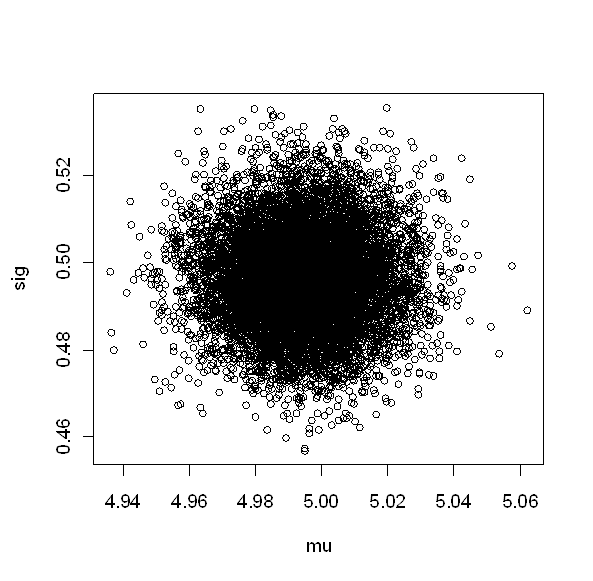
\includegraphics[height=3in]{Ch6/figs/postdist}
\end{center}
\caption{Joint posterior distribution of mu and sig from a Normal Model}
\label{postdist.fig}
\end{figure}

\begin{figure}
\begin{center}
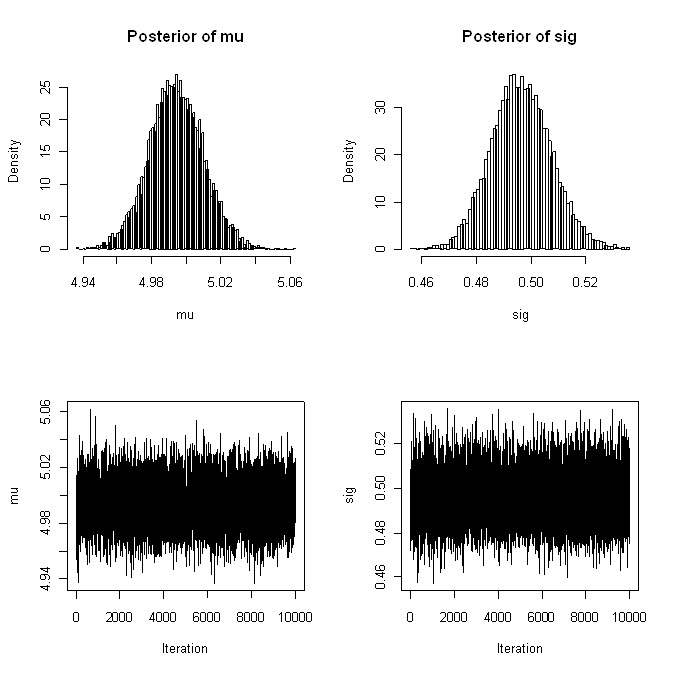
\includegraphics[width=2.5in]{Ch6/figs/plotsofPD}
\end{center}
\caption{Plots of the posterior distributions of $\mu$ (a) and $\sigma$ (b)
  from a Normal model and time series plots of $\mu$ (c) and $\sigma$ (d).}
\label{plotsofPD.fig}
\end{figure}

\subsection{ Metropolis-Hastings sampling   }

Although it is applicable to a wide range of problems, the limitations
of Gibbs sampling are immediately obvious – what if we do not want to
use conjugate priors (or what if we cannot recognize the full
conditional distribution as a parametric distribution, or simply do
not want to worry about these issues)? The most general solution is to
use the Metropolis-Hastings (MH) algorithm, which also goes back to
the work by \citet{metropolis_ulam:1953}. You saw the basics of this
algorithm in Chapter 2. In a nutshell, because we do not recognize the
posterior $p(\theta|y)$ as a parametric distribution, the MH algorithm
generates samples from a known proposal distribution, say $h(\theta)$,
that depends on $\theta$ at $t-1$. The $t^{th}$ sample is accepted with probability. 

\[
r = \frac{ f(\theta^{(t-1)}) h(\theta^{(t)}|\theta^{(t-1)})}
    {f(\theta^{(t)}) h(\theta^{(t-1)}|\theta^{(t)}) }
\]

Proposal distributions can be absolutely
anything!  You can generate candidate values from a $normal(0,1)$
distribution, from a uniform(-3455,3455) distribution, or anything of
proper support.  Note, however, that good choices of $h()$ are those
that approximate the posterior distribution. Obviously if $h() =
f(\theta|y)$ (i.e., the posterior) then you always accept the draw,
and it stands to reason that proposals that are more similar to
$f(\theta|y)$ will lead to higher acceptance probabilities. 

The original Metropolis algorithm
required $h(\theta)$ to be symmetric so that
$h(\theta^{(t)}|\theta^{(t-1)}) = h(\theta^{(t-1)}|\theta^{(t)})$. 
In that case these two terms just cancel
out from the MH acceptance probability and $r$ is then just the ratio
of the target density evaluated at the candidate value to that
evaluated at the current value. A later
development of the algorithm by \citet{hastings:1970} lifted this
condition. 
Since using a symmetric proposal distribution makes life a little
easier, we are going to focus on this specific case. A type of symmetric proposal useful in many situations is the
so-called {\it random-walk} proposal distribution where candidate values
are drawn from a normal distribution with mean equal to the current
value and some standard deviation, say $\delta$, which is prescribed by
the user (see below for further explanation). 

{\bf Parameters with bounded support}: Many models contain parameters that
have  bounded support. E.g., variance parameters live on $[0,\infty]$,
parameters that represent probabilities live on $[0,1]$, etc..
 In that case it is sometimes convenient to use a random
walk proposal distribution that can generate any real number (e.g., a
normal random walk proposal). In that case,
we can just reject parameters that are
outside of the parameter space (XXXX REF FOR THIS XXXX).

It is worth
knowing that there are alternatives to the random walk MH algorithm. For
example, in the independent M-H, $\theta^{(t)}$ does not depend on
$\theta^{(t-1)}$, while the Langevin algorithm \citep{roberts_etal:1998}
aims at avoiding the random walk by favoring moves towards regions of
higher posterior probability density. The interested reader should
look up these algorithms in \citet{robert_casella:2004} or
\citet{robert_casella:2010}.

Building a MH sampler can be broken down into several steps. We are going to demonstrate these steps using a different but still simple and common model – the logit-normal or logistic regression model. For simplicity, assume that
\[
y \sim \mbox{Bern}(\exp(\theta)/(1+ exp(\theta)))
\]
and
\[
\theta \sim \mbox{Normal}(\mu, \sigma)
\]
The following steps are required to set up a random walk MH algorithm:

{\flushleft Step 0: Choose initial values, $\theta^{(0)}$.}

{\flushleft Step 1: Generate a proposed value of $\theta$ at $t$ from $h(\theta^{(t)}|\theta^{(t-1)})$. }
We often use a Normal proposal distribution, so we draw $\theta^{(1)}$ from $Normal(\theta^{(0)}, \delta)$, where $\delta$ is the variance of the Normal proposal distribution, the tuning parameter that we have to set.

{\flushleft Step 2: Calculate the ratio of posterior densities for the proposed and the original value for $\theta$: }
\[
r = \frac{p(\theta^{(t)}|y)}  {p(\theta^{(t-1)}|y)}
\]
In our example,
\[
r = \frac{\mbox{Bernoulli}(y|\theta^{(t)}) * Normal(\theta^{(t)}|\mu, \sigma)} {Bernoulli(y|\theta^{(t-1)}) * Normal(\theta^{(t-1)}|\mu, \sigma)}
\]
Step 3: Set

\begin{eqnarray*}
\theta^{(t)}  &= &   \theta^{(t)} \mbox{with probability min(r,1)}\\
	 & = & 	\theta^{(t-1)} \mbox{ otherwise }
\end{eqnarray*}

%should work now


We can do that by drawing a random number $u$ from a
$\mbox{Unif}(0,1)$ and accept $\theta^{(t)}$ if
$u<r$.
Repeat for $t = 1,2,\ldots$ a large number of samples.
The {\bf R} code for this MH sampler is provided in Panel 2 XXXX.
{\small
\begin{verbatim}
Panel 2: R code to run a Metropolis sampler on a simple Logit-Normal model.

Logreg.MH<-function(y=y, mu0=mu0, sig0=sig0, niter=niter) {

out<-c()

theta<-runif(1, -3,3) #initial value

for (iter in 1:niter){
theta.cand<-rnorm(1, theta, 0.2)

loglike<-sum(dbinom(y, 1, exp(theta)/(1+exp(theta)), log=TRUE))
logprior <- dnorm(theta,mu0 ,sig0, log=TRUE)
loglike.cand<-sum(dbinom(y, 1, exp(theta.cand)/(1+exp(theta.cand)), log=TRUE))
logprior.cand <- dnorm(theta.cand, mu0, sig0, log=TRUE)

if (runif(1)<exp((loglike.cand+logprior.cand)-(loglike+logprior))){
theta<-theta.cand
}
out[iter]<-theta
}

return(out)
}
\end{verbatim}
}

The reason we sum the logs of the likelihood and the prior, rather than multiplying the original values, is simply computational. The product of small probabilities can be numbers very close to 0, which computers do not handle well. Thus we add the logarithms, sum, and exponentiate to achieve the desired result. Similarly, in case you have forgotten some elementary math, $x/y = exp(log(x)-log(y))$, with the latter being favored for computational reasons.

Comparing MH sampling to Gibbs sampling, where all draws from the conditional distribution are used, in the MH algorithm we discard a portion of the candidate values, which inherently makes in less efficient than Gibbs sampling – the price you pay for its increased generality.
In Step 1 of the MH sampler we had to choose a variance, $\delta$, for the Normal proposal distribution. Choice of the parameters that define our candidate distribution is also referred to as 'tuning', and it is important since adequate tuning will make your algorithm more efficient. 
$\delta$ should be chosen (a) large enough so that each step of drawing a new proposal value for $\theta$ can cover a reasonable distance in the parameter space, as otherwise, mixing of the Markov chain is inefficient and chains will tend to have strong autocorrelation; and (b) small enough so that proposal values are not rejected too often, as otherwise the random walk will 'get stuck' at specific values for too long.  As a rule of thumb, your candidate value should be accepted in about 40\% of all cases. Acceptance rates of 20 -- 80\% are probably ok, but anything below or above may well render your algorithm inefficient (this does not mean that it will give you wrong results – only that you will need more iterations to converge to the posterior distribution). In practice, tuning will require some 'trial-and-error' and some common sense. Or, one can use an adaptive phase, where the tuning parameter is automatically adjusted until it reaches a user-defined acceptance rate, at which point the adaptive phase ends and the actual Markov chain begins. This is computationally a little more advanced. \citet{link_barker:2009} discuss this in more detail. It is important the samples drawn during the adaptive phase are discarded.
To illustrate the effects of tuning, we ran the Metropolis-within-Gibbs algorithm in Panel 2 XX with $\delta=0.01$, $\delta=0.2$ and $\delta=1$. The first 150 iterations for $\theta$ are shown in Fig. \ref{mcmc.fig.tuning}. We see that for a very small $\delta$ (the dashed line) the burn-in is extremely slow - after 150 iterations the chain isn't even half way there, while for the other two values of $\delta$ (solid and dotted)the burn-in phase seems to be over after only about 10 iterations. While $\delta=0.2$ leads to reasonably good mixing, the chain clearly gets stuck on certain values with $\delta=1$.
%'tuning' is a new figure I made... don't know about the size specifications, just copied those from another picture. Do you set them at 
%the actual size of the figure or the size you want it to be??
 \begin{figure}
\begin{center}
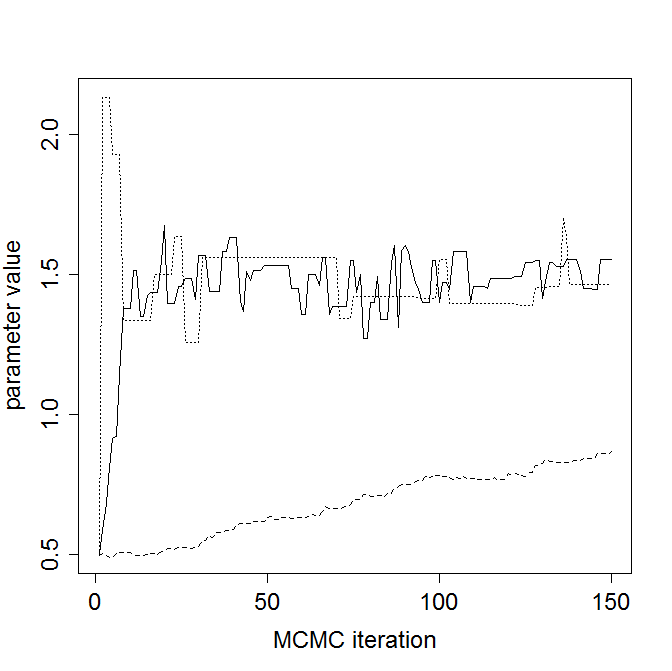
\includegraphics[height=3in,width=4in]{Ch6/figs/tuning}
\end{center}
\caption{Time series plots of $\theta$ from a MH algorithm with tuning parameter  $\delta = 0.01$ (dashed line), 0.2 (solid line) and  1 (dotted line).}
\label{mcmc.fig.tuning}
\end{figure}

Other than graphically, you can easily check acceptance rates for the parameters you monitor (that are part of your output) using the rejectionRate() function of the package coda (we will talk more about this package a little later on). Do not let the term 'rejection rate' confuse you; it is simply 1 -- acceptance rate. There may be parameters – for example, individual values of a random effect or latent variables – that you do not want to save, though, and in our next example we will show you a way to monitor their acceptance rates with a few extra lines of code.



\subsection{ Metropolis-within-Gibbs }

One weakness of the MH sampler is that formulating the joint posterior when evaluating whether to accept or reject the candidate values for $\theta$ becomes increasingly complex or inefficient as the number of parameters in a model increases. As you already saw in Chapter 2, in these cases you can simply combine MH sampling and Gibbs sampling. You can use Gibbs sampling to break down your high-dimensional parameter space into easy-to-handle one-dimensional conditional distributions and use MH sampling for these conditional distributions. Better yet – if you have some conjugacy in your model, you can use the more efficient Gibbs sampling for these parameters and one-dimensional MH for all the others. You have already seen the basics of how to build both types of algorithms, so we can jump straight into an example here and build a Metropolis-within-Gibbs algorithm.

\section{ GLMMs – Poisson regression with a random effect }

Let's assume a model that gets us closer to the problem we ultimately want to deal with – a GLMM. Here, we assume we have Poisson counts, $y$, from $i$ plots in $j$ different study sites, and we believe that the counts are influenced by some plot-specific covariate, $x$, but that there is also a random site effect. So our model is:
\[
y_{ij} \sim Poisson (\lambda_{ij})
\]
\[
\lambda_{ij} = exp (a_j + bx_i)
\]
Let's use Normal priors on $a$ and $b$,  \[
a_j \sim Normal (\mu_a, \sigma_a)
\]
and
\[
b \sim Normal (\mu_b, \sigma_b)
\].

Since we want to estimate the random effect in this model, we do not
specify $\mu_a$ and $\sigma_a$, but instead, estimate them as well, so we have
to specify hyperpriors for these parameters:
\begin{eqnarray*}
\mu_a  &\sim &  Normal(\mu_0, \sigma_0)  \\
\sigma_{a} & \sim & InvGamma(a_0, b_0)
\end{eqnarray*}
%In this entire section below I am unsure of the indexing of a, y and x. I know what I'm trying to say but I'm not sure I'm saying it correctly... could someone please check? So what I am trying to say, for example in the expression for a1 (a at j=1), is that you need all the yi's at j=1, and all the x at j=1.
With the model fully specified, we can compile the full conditionals, breaking the multi-dimensional parameter space into one-dimensional components:

%%this works but it doesn't look paritcularly pretty
\begin{equation*}
\begin{split}
p(a_1|a_2,a_3,\ldots,a_j,b,y)& \propto   p(y_{i1}|a_1,b) * p(a_1) \\
	 & \propto    Poisson(y_{i1}| exp(a_1 + bx_i))\\
     & \quad * Normal(a_1|\mu_a, \sigma_a)
\end{split}
\end{equation*}

\begin{verbatim}
\begin{eqnarray*}
p(a_2|a_1,a_3,\ldots,a_j,b,y) & \propto&  p(y_{i2}|a_2,b) * p(a_2) \\
	 & \propto  & Poisson(y_{i2}|exp(a_2 + bx_i)) * Normal(a_2|\mu_a, \sigma_a)
\end{eqnarray}
and so on for all elements of a.
\begin{eqnarray*}
p(b|a,y) &\propto & p(y|a,b) * p(b) \\
	 &\propto& Poisson(y|exp(a + bx)) *Normal(b|\mu_b, \sigma_b)
\end{eqnarray*}
\end{verbatim}
%couldn't get this to work either

Finally, we need to update the hyperparameters for a:
\[
p(\mu_a|a) \propto p(a|\mu_a, \sigma_a) *p(\mu_a)
\]
\[
p(\sigma_a|a) \propto p(a|\mu_a, \sigma_a) *p(\sigma_a)
\]
Since we assumed $a$ to come from a Normal distribution, the choice of priors for $\mu_a$ (Normal) and $\sigma_a$ (Inverse Gamma) leads to the same conjucagy we observed in our initial Normal model, so that both hyperparameters can be updated using Gibbs sampling.

Now let's build the updating steps for these full conditionals. Again, for the MH steps that update $a$ and $b$ we use Normal proposal distributions with standard deviations $\delta_{a}$ and $\delta_{b}$.

First, we set the initial values $a^{(0)}$ and $b^{(0)}$. Then, starting with $a_1$, we draw $a_1^{(1)}$ from $Normal (a_1^{(0)}, \delta_{a})$, calculate the conditional posterior density of $a_1^{(0)}$ and $a_1^{(1)}$  and compare their ratios,
\[
r = \frac{Poisson(y_{i1}|exp(a_1^{(1)} + bx_i)) * Normal(a_1^{(1)}|\mu_a, \sigma_a)} {Poisson(y_{i1}|exp(a_1^{(0)} + bx_i)) * Normal(a_1^{(0)}|\mu_a, \sigma_a)}
\]
and accept $a_1^{(1)}$ with probability $min(r,1)$. We repeat this for all a's.

For $b$, we draw $b_1^{(1)}$ from $Normal (b^{(0)}, \delta_{b})$, compare the posterior densities of $b^{(0)}$ and $b^{(1)}$,
\[
r = \frac{Poisson(y|exp(a + b_1^{(1)}x)) *Normal(b_1^{(1)}|\mu_b, \sigma_b)} { Poisson(y|exp(a + b_1^{(0)}x)) *Normal(b_1^{(0)}|\mu_b, \sigma_b)},
\]
and accept $b_1^{(1)}$  with probability $min(r,1)$.

For $\mu_a$ and $\sigma_a$, we sample directly from the full conditional distributions (Eq. \ref{XX}  and Eq. \ref{XX}):
\[
\mu_a^{(1)} \sim Normal (\mu_n, \sigma_n)
\]
where 
\[\mu_n =  \frac{\sigma_a^{(0)}}  {\sigma_a^{(0)}   +n_a  *  \sigma_0} *  \mu_0 +  \frac{n_a * \sigma_0} {\sigma_a^{(0)}   +n_a* \sigma_0} *\bar{a}^{(1)}
\]
and 

\[
\sigma_n= \frac{\sigma_a^{(0)}  * \sigma_0 } {\sigma_a^{(0)}  + n* \sigma_0}
\]
Here, $\bar{a}$ is the current mean of the vector $\bf{a}$, which we updated before, and $n_a$ is the length of $\bf{a}$. For $\sigma_a$ we use $\sigma_a^{(1)}\sim Inv Gamma (a_n, b_n)$,
where  $a_n = n_a/2   + a_0$, and $b_n = 0.5 ( \displaystyle\sum\limits_{j=1}^{n_a} a_j^{(1)}-\mu_a^{(1)})^2+ b_0$.

We repeat these steps over $T$ iterations of the MCMC algorithm.
In this example we may not want to save each individual $a$, but are only interested in their mean and standard deviation. Since these two parameters will change as soon as the value for one element in $\bf{a}$ changes, their acceptance rates will always be close to 1 and are not representative of how well your algorithm performs. To monitor the acceptance rates of parameters you do not want to save, you simply need to add a few lines of code into your updater to see how often the individual parameters are accepted. The full code for the MCMC algorithm of our Poisson GLMM in Panel 3 (XXX) shows one way how to monitor acceptance of individual $a$'s.

{\small
\begin{verbatim}
Panel 3: R code for the Metropolis-within-Gibbs sampler for
a Poisson regression with random intercepts.

Pois.reg<-function(y=y,site=site,mu0=mu0,sig0=sig0,a0=a0,b0=b0,
          mub=mub, sigb=sigb, niter=niter){

lev<-length(unique(site))     #number of sites
a<-runif(lev,-5,5)		#initial values a
b<-runif(1,0,5)			#initial value b
mua<-mean(a)
siga<-sd(a)

out<-matrix(nrow=niter, ncol=3)
colnames(out)<-c('mua','siga','b')

for (iter in 1:niter) {

#update a
aUps<-0			  #initiate counter for acceptance rate of a
for (j in 1:lev) { 	  #loop over sites
a.cand<-rnorm(1, a[j], 0.1)	#update intercepts a one at a time
loglike<- sum(dpois (y[site==j], exp(a[j] + b*x[site==j]), log=TRUE))
logprior<- dnorm(a[j], mua,siga, log=TRUE)
loglike.cand<- sum(dpois (y[site==j], exp(a.cand + b *x[site==j]), log=TRUE))
logprior.cand<- dnorm(a.cand,  mua,siga, log=TRUE)
if (runif(1)< exp((loglike.cand+logprior.cand) –(loglike+logprior))) {
a[j]<-a.cand
aUps<-aUps+1
}
}

if(iter %% 100 == 0) {  #this lets you check the acceptance rate of a at every 100th iteration
            cat("   Acceptance rates\n")
            cat("     a =", aUps/lev, "\n")
}

#update b
b.cand<-rnorm(1, b, 0.1)
avec<-rep(a, times=c(rep(10,10)))
loglike<- sum(dpois (y, exp(avec + b*x), log=TRUE))
logprior<- dnorm(b, mub,sigb, log=TRUE)
loglike.cand<- sum(dpois (y, exp(avec + b.cand *x), log=TRUE))
logprior.cand<- dunif(b.cand, mub,sigb, log=TRUE)
if (runif(1)< exp((loglike.cand+logprior.cand) – (loglike+logprior) )) {
b<-b.cand
}

#update mua using Gibbs sampling
abar<-mean(a)
mun<- (siga/(siga+lev*sig0))*mu0 + (lev*sig0/(siga+lev* sig0))*abar
sign <- (siga*sig0)/ (siga+lev*sig0)
mua<-rnorm(1,mun, sqrt(sign))

#update siga using Gibbs sampling
a0n<-lev/2 + a0
b0n<- 0.5 * (sum((a-mua)^2)) +b0
siga<-1/rgamma(1,shape=a0n, rate=b0n)

out[iter,]<-c(mua, sqrt(siga), b)

}

return(out)
}
\end{verbatim}
}

\subsection{Rejection sampling and slice sampling }

While MH and Gibbs sampling are probably the most widely applied algorithms for posterior approximation, there are other options that work under certain circumstances and may be more efficient when applicable. WinBUGS applies these algorithms and we want you to be aware that there is more out there to approximate posterior distributions than Gibbs and MH.
One alternative algorithm is rejection sampling. Rejection sampling is not an MCMC method, since each draw is independent of the others. The method can be used when the posterior $p(\theta|y)$ is not a known parametric distribution but can be expressed in closed form. Then, we can use a so-called envelope function, say, $g(\theta)$, that we can easily sample from, with the restriction that $p(\theta|y) < M * g(\theta)$. We then sample a candidate value for $\theta$ from $g(\theta)$, calculate $r = p(\theta|y)/M*g(\theta)$ and keep the sample with the probability $r$. $M$ is a constant that has to be picked so that $r$ lies between 0 and 1, for example by evaluating both $p(\theta|y)$ and $g(\theta)$ at $n$ points and looking at their ratios. Rejection sampling only works well if $g(\theta)$ is similar to $p(\theta|y)$, and packages like WinBUGS use adaptive rejection sampling \citep{gilks_wild:1992}, where a complex algorithm is used to fit an adequate and efficient $g(\theta)$ based on the first few draws. Though efficient in some situations, rejection sampling does not work well with high-dimensional problems, since it becomes increasingly hard to define a reasonable envelope function. For an example of rejection sampling in the context of SCR models, see Chapter 9 XXXX.
Another alternative is slice sampling \citep{neal:2003}. In slice sampling, we sample uniformly from the area under the plot of $p(\theta|y)$. Considering a single univariate theta. Let's define an auxiliary variable, $U \sim  Uniform(0, p(\theta|y))$. Then, $\theta$ can be sampled from the vertical slice of $p(\theta|y)$ at $U$ (Figure 4):

\[
\theta|U \sim \mbox{Unif}(B),
\]
where $B = \{\theta: p(\theta|y) \geq U\}$
%do these symbols mean  'B is element of the interval of all theta for which p(theta) is larger than or equal to U?' 

\begin{figure}
\begin{center}
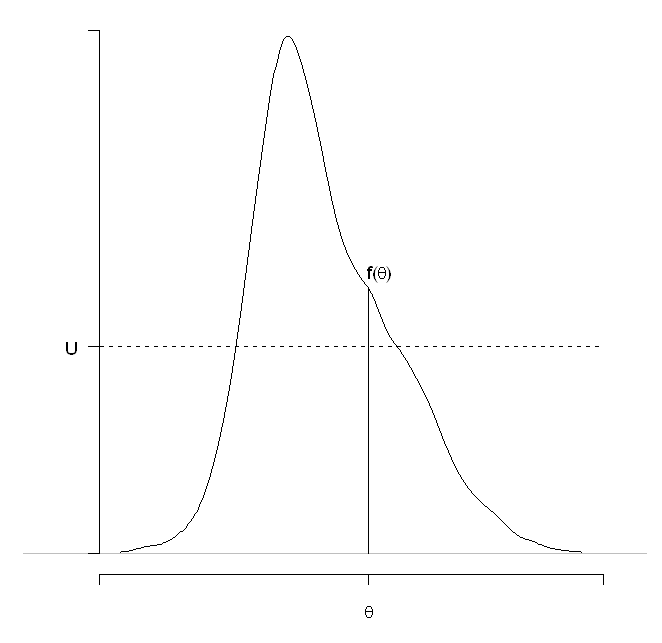
\includegraphics[height=2in]{Ch6/figs/slicesampling}
\end{center}
\caption{Slice sampling. For...}
\label{slicesample.fig}
\end{figure}

\footnote{there are supposed to be equations in the caption of figure
4 but it kept causing errors}

Slice sampling can be applied in many situations; however, implementing an efficient slice sampling procedure can be complicated. We refer the interested reader to chapter 7 of \citet{robert_casella:2010} for a simple example.
Both rejection sampling and slice sampling can be applied on one-dimensional conditional distributions within a Gibbs sampling setup.

\section{MCMC for closed capture-recapture Model Mh}
\subsection{Building your own MCMC algorithm}

By now you have seen MCMC samplers for some simple GL(M)M's. Now, to ease you into more complex models, we construct our own MCMC algorithm using a Metropolis-within-Gibbs sampler for the non-spatial Model with individual heterogeneity in capture probability $M_{h}$, developed in Chapt. \ref{chapt.closed}. 

To recapitulate: Under the non-spatial model, each of the $n$ observed individuals is either detected (1) or not (0) during each of $K$ sampling occasions. We estimate $N$ using data augmentation and have a Bernoulli model for the
zero-inflation variables $z_{i}$. The binomial observation model
is expressed conditional on the latent variables
$z_{i}$. Further, we
prescribe a distribution for the capture probability $p_{i}$. Here we assume
\[
\mathrm{logit}(p_{i}) \sim \mbox{Normal}(\mu,\sigma^2)
\]


As usual, we will have to go through two general steps before we write the MCMC algorithm:

(1)Identify your model with all its components (including
    priors)

(2) Recognize and express the full conditional distributions for
    all parameters
    
Our model components are as follows: $[y_{i}| p_{i},z_{i}]$,
$[p_{i}|\mu_{p},\sigma_{p}]$, and $[z_{i}|\psi]$
for {\it each} $i=1,2,\ldots,M$ and then prior distributions
$[\mu_{p}]$, $[\sigma_{p}]$ and $[\psi]$.
The joint posterior distribution of all unknown quantities in the model
is proportional to the joint distribution of all elements
$y_{i},p_{i},z_{i}$ and also the prior distributions of the prior parameters:
\[
\left\{ \prod_{i=1}^{M} [y_{i}|p_{i},z_{i}][p_{i}|\mu_{p},\sigma_{p}]
[z_{i}|\psi] \right\} [\mu_{p},\sigma_{p},\psi]
\]
For prior distributions, we assume that $\mu_{p},\sigma_{p}, \psi$ are
mutually independent and for $\mu_{p}$ and $\sigma_{p}$ we use
improper uniform priors, and $\psi \sim \mbox{Unif}(0,1)$.  Note that
the likelihood contribution for each individual, when conditioned on
$p_{i}$ and $z_{i}$, does not depend on $\psi$, $\mu_{p}$, or
$\sigma_{p}$.  As such, the full-conditionals for the structural
parameters $\psi$ only depends on the collection of data augmentation
variables $z_{i}$, and that for $\mu_{p}$ and $\sigma_{p}$ will only
depends on the collection of latent variables $p_{i}; i=1,2,\ldots,M$.
The full conditionals for all the unknowns are as follows:

{\bf (1)} For $p_{i}$:
\begin{eqnarray*}
[p_{i}|y_{i}, \mu_p, \sigma_{p},z_{i}=1] &\propto  &
[y_{i}|p_{i}][p_{i}|\mu_p,\sigma_{p}^{2}] \mbox{ if $z_{i}=1$ }  \\
                 &  &  [p_{i}|\mu_p,\sigma_{p}] \mbox{ if $z_{i}=0$ }
\end{eqnarray*}

{\bf (2)} for $z_{i}$:
\[
z_{i} | \cdot \propto [y_{i}|z_{i}*p_{i}] \mbox{Bern}(z_{i}|\psi)
\]

{\bf (3)} For $\mu_{p}$:
\[
[\mu_{p} | \cdot ] \sim \prod_{i} [p_{i}| \cdot] *\mbox{const}
\]


{\bf (4)} For $\sigma_{p}$:
\[
[ \sigma_{p}|\cdot ] \sim\prod_{i}[p_{i}| \cdot ]*\mbox{const}
\]

{\bf (5)} For $\psi$:
\[
\psi|\cdot\sim \mbox{Beta}(1 + \sum z_{i}, 1 + M - \sum z_{i})
\]


What we've done here is identify each of the full conditional
distributions in sufficient detail to toss them into our
Metropolis-Hastings algorithm. With the exception of $\psi$ which has
a convenient analytic solution -- it is a beta distribution which we
can easily sample directly. In truth, we could also sample $\mu_{p}$
and $\sigma_{p}^{2}$ directly with certain choices of prior
distributions. For example, if $\mu_{p} \sim \mbox{Normal}(0, 1000)$
then the full conditional for $\mu_{p}$ is also normal, etc..
We implement an MCMC algorithm for this model in the following block
of {\bf R} code.  
%Andy, I think we should edit code so it's comparable to the rest in this chapter (eg loglik instead of lik.curr etc. 
%Should I do this in here or do you have an R script file for this code that's goint in the scrbook package? Then, I'd probably better
% edit the .R file and paste it in here so they match.
\begin{verbatim}

## obtain the bear data by executing the previous data grabbing
## function

temp<-getdata()
M<-temp$M
K<-temp$K
ytot<-temp$ytot


###
### MCMC algorithm for Model Mh

out<-matrix(NA,nrow=100000,ncol=4)
dimnames(out)<-list(NULL,c("mu","sigma","psi","N"))
lp<- rnorm(M,-1,1)
p<-expit(lp)
mu<- -1
p0<-exp(mu)/(1+exp(mu))
sigma<- 1
psi<- .5
z<-rbinom(M,1,psi)
z[ytot>0]<-1

for(i in 1:100000){

### update the logit(p) parameters
lp.cand<- rnorm(M,lp,1)  # 0.5 is a tuning parameter
p.cand<-expit(lp.cand)
lik.curr<-log(dbinom(ytot,K,z*p)*dnorm(lp,mu,sigma))
lik.cand<-log(dbinom(ytot,K,z*pc)*dnorm(lpc,mu,sigma))
kp<- runif(M) < exp(lik.cand-lik.curr)
p[kp]<-pc[kp]
lp[kp]<-lpc[kp]

p0c<- rnorm(1,p0,.05)
if(p0c>0 & p0c<1){
muc<-log(p0c/(1-p0c))
lik.curr<-sum(dnorm(lp,mu,sigma,log=TRUE))
lik.cand<-sum(dnorm(lp,muc,sigma,log=TRUE))
if(runif(1)<exp(lik.cand-lik.curr)) {
 mu<-muc
 p0<-p0c
}
}

sigmac<-rnorm(1,sigma,.5)
if(sigmac>0){
lik.curr<-sum(dnorm(lp,mu,sigma,log=TRUE))
lik.cand<-sum(dnorm(lp,mu,sigmac,log=TRUE))
if(runif(1)<exp(lik.cand-lik.curr))
 sigma<-sigmac
}

### update the z[i] variables
zc<-  ifelse(z==1,0,1)  # candidate is 0 if current = 1, etc..
lik.curr<- dbinom(ytot,K,z*p)*dbinom(z,1,psi)
lik.cand<- dbinom(ytot,K,zc*p)*dbinom(zc,1,psi)
kp<- runif(M) <  (lik.cand/lik.curr)
z[kp]<- zc[kp]

psi<-rbeta(1, sum(z) + 1, M-sum(z) + 1)

out[i,]<- c(mu,sigma,psi,sum(z))
}
\end{verbatim}



{\bf Remarks}: (1) for parameters with bounded support, i.e.,
$\sigma_{p}$ and $p_{0}$, we are using a random walk candidate
generator but rejecting draws outside of the parameter space.  (2) We
mostly use Metropolis-Hastings except for the data augmentation
parameter $\psi$ which we sample directly from its full-conditional
distribution which is a beta distribution.  (3) Even the latent data
augmentation variables $z_{i}$ are updated using Metropolis-Hastings
although they too can be updated directly from their full-conditional.

\section{MCMC algorithm for the basic spatial capture-recapture model}

Conceptually, but also in terms of MCMC coding, it is only a small step from the non-spatial model Mh to a fully spatial capture-recapture model. Next, we'll walk you through the steps of building your own MCMC sampler for the basic SCR model (i.e. without any individual, site or time specific covariates) with both a Poisson and a binomial encounter process.
As usual, we will have to go through two general steps before we write the MCMC algorithm:

(1)Identify your model with all its components (including
    priors)

(2) Recognize and express the full conditional distributions for
    all parameters

It is worthwhile to go through all of step 1 for an SCR model, but you
have probably seen enough of step 2 in our previous examples to get
the essence of how to express a full conditional
distribution. Therefore, we will exemplify step 2 for some parameters
and tie these examples directly to the respective R code.


{\bf Step 1 -- Identify your model}

Recall the components of the basic SCR model with a Poisson encounter process from Chapt. \ref{XX}:
We assume that individuals $i$, or rather, their activity centers $s_i$, are uniformly distributed across our state space $S$,
\[
s_i  \sim U(S)
\]
and that the number of times individual $i$ encounters trap $j$, $y_{ij}$, is a random Poisson variable with mean $\lambda_{ij}$,
\[
y_{ij} \sim Poisson(\lambda_{ij})
\]
The tie between individual location, movement and trap encounter rates is made by the assumption that $\lambda_{ij}$, is a decreasing function of the distance between $s_i$ and $j$, $D_{ij}$, of the half-normal form
\[
\lambda_{ij} =  \lambda_0 * exp(-D_{ij}^2/2\sigma^2),
\]
where $\lambda_0$ is the baseline trap encounter rate at $Dij=0$ and $\sigma$ controls the shape of the half-normal function.

In order to estimate the number of $s_i$ in $S$, $N$, we use data augmentation (Sect. \ref{3.XYZ}) and create $M-n$ all-0 encounter histories, where $n$ is the number of individuals we observed and $M$ is an arbitrary number that is larger than $N$. We estimate $N$ by summing over the auxiliary data augmentation variables, $z_i$, which is 1 if the individual is part of the population and 0 if not, and assume that $z_i$ is a random Bernoulli variable,
\[
z_{i} \sim \mbox{Bern}(\psi)
\]


To link the two model components, we modify our trap encounter model to
\[
\lambda_{ij} = \lambda_0 * exp(-D_{ij}^2/2\sigma^2) * z_{i}.
\]
The model has the following structural parameters, for which we need to specify priors:

$\psi$: the $Uniform (0,1)$ is required as part of the data augmentation procedure and in general is a natural choice of an uninformative prior for a probability; note that this is equivalent to a $Beta(1,1)$ prior, which will come in handy later.

$s_{i}$: since $s_{i}$ is a pair of coordinates it is two-dimensional and we use a uniform prior limited by the extent of our state-space over both dimensions.

$\sigma$: we can conceive several priors for $\sigma$ but let's assume an improper prior, one that is Uniform over $(-Inf, Inf)$. We will see why this is convenient when we construct the full conditionals for $\sigma$.

$\lambda_{0}$: analogous, we will use a $Uniform (-Inf, Inf)$ improper prior for $\lambda_{0}$.

The parameter that is the objective of our modeling, $N$, is a derived parameter that we can simply obtain by summing all $z_i$:
\[
N=\sum(z)
\]


{\bf Step 2 -- Construct the full conditionals}
Having completed step 1, let's look at the full conditional distributions for some of these parameters.
We find that with improper priors, full conditionals are proportional only to the likelihood of the observations; for example, take the movement parameter $\sigma$:
\[
[\sigma|s, \lambda_{0}, z, y] \propto [y| s, \lambda_{0}, z, \sigma] * [\sigma]
\]
Since the improper prior implies that $[\sigma] \propto 1$, we can reduce this further to
\[
[\sigma|s, \lambda_{0}, z, y] \propto [y| s, \lambda_{0}, z, \sigma]
\]
The R code to update $\sigma$ is shown in Panel 4. Notice that we automatically reject negative candidate values, since $\sigma$ cannot be $<0$.  

{\small
\begin{verbatim}
Panel 4: R code to update sigma within an MCMC algorithm for
an SCR model when using an improper prior


sig.cand <- rnorm(1, sigma, 0.1)	#draw candidate value
 if(sig.cand>0){   #automatically reject sig.cand that are <0
     lam.cand <- lam0*exp(-(D*D)/(2*sig.cand*sig.cand))
     ll<- sum(dpois(y, lam*z, log=TRUE))
     llcand <- sum(dpois(y, lam.cand*z, log=TRUE))
     if(runif(1) < exp( llcand  - ll) ){
         ll<-llcand
         lam<-lam.cand
         sigma<-sig.cand
      }
  }

\end{verbatim}
}
These steps are analogous for  $\lambda_{0}$ and $s_i$ and we will use MH steps for
all of these parameters. Similar to the random intercepts in our
Poisson GLMM, we update each $s_i$ individually. Note that to be fully
correct, the full conditional for $s_i$ contains both the likelihood and
prior component, since we did not specify an improper, but a Uniform
prior on $s_i$. However, with a Uniform distribution the probability
density of any value is 1/(upper limit - lower limit) =
constant. Thus, the prior components are identical for both the
current and the candidate value and can be ignored (formally, when you
calculate the ratio of posterior densities, $r$, the identical prior
component appears both in the numerator and denominator, so that they
cancel each other out).

We still have to update $z_i$. The full conditional for $z_i$ is
\[
[z_i|y, \sigma, \lambda_0, s] \propto [y|z,\sigma, \lambda_0, s] * [z_i]
\]
and since $z_i \sim Bernoulli(\psi)$,
the term has to be taken into account when updating $z_i$. The R code for updating $z_i$ is shown in Panel 5.

{\small
\begin{verbatim}
Panel 5: R code to update z…

        zUps <- 0		#set counter to monitor acceptance rate
        for(i in 1:M) {
            if(seen[i])	#no need to update seen individuals, since their z =1
                next
            zcand <- ifelse(z[i]==0, 1, 0)
            llz <- sum(dpois(y[i,],lam[i,]*z[i], log=TRUE))
            llcand <- sum(dpois(y[i,], lam[i,]*zcand, log=TRUE))

            prior <- dbinom(z[i], 1, psi, log=TRUE)
            prior.cand <- dbinom(zcand, 1, psi, log=TRUE)
            if(runif(1) < exp( (llcand+prior.cand) - (llz+prior) )) {
                z[i] <- zcand
                zUps <- zUps+1
            }
        }
\end{verbatim}
}

$\psi$
itself is a hyperparameter of the model, with an uninformative prior distribution of $Unif(0,1)$ or $Beta(1,1)$, so that
\[
\psi|z \propto [z|\psi] * Beta(1,1)
\]
The Beta distribution is the conjugate prior to the Binomial and Bernoulli distributions (remember that $z \sim Bernoulli(\psi))$. The general form of a full conditional of a Beta-Binomial model with $yi \sim Bernoulli (p) $ and $p \sim Beta(a,b) $ is
\[
p(p|y) \propto Beta(a + \sum y_i, b + n-\sum y_i)
\]
In our case, this means we update psi as follows:
\begin{verbatim}
si<-rbeta(1, 1+sum(z), 1 + M-sum(z))
\end{verbatim}

These are all the building blocks you need to write the MCMC algorithm
for the spatial null model with a Poisson encounter process.  You can
find the full R code (SCR0pois.R) in the R package scrbook XXXXXX.

\subsection{SCR model with binomial encounter process}
The equivalent SCR model with a binomial encounter process is very similar. Here, each individual $i$ can only be detected once at any given trap $j$ during a sampling occasion $k$.
Thus
\[
y_{ij} \sim Binomial (p_{ij}, K)
\]
Where $p_{ij}$ is some function of distance between ${\bf s}_{i}$ and trap location ${\bf x}_{j}$. Here we use:
\[
p_{ij}=1-exp(-\lambda_{ij})
\]
Recall from Chapter 2 that this is the complementary log-log (cloglog) link function, which constrains $p_{ij}$ to fall between 0 and 1.
For our MCMC algorithm that means that, instead of using a Poisson likelihood, $Poisson(y|\sigma,\lambda_0,s,z)$, we use a Binomial likelihood, $Binomial(y,K|\sigma,\lambda_0,s,z)$, in all the conditional distributions. As an example, Panel 6 shows the updating step for $\lambda_0$ under a binomial encounter model. The full MCMC code for the binomial SCR (SCR0binom.R) can be found in the R package scrbook XXXXXX.

{\small
\begin{verbatim}
Panel 6: MCMC updater for lam0 in a SCR model with Binomial encounter
process and cloglog link function on detection. Here, pmat =
1-exp(-lam).

        lam0.cand <- rnorm(1, lam0, 0.1)
        if(lam0.cand >0){   #automatically reject lam0.cand that are <0
            lam.cand <- lam0.cand*exp(-(D*D)/(2*sigma*sigma))
            p.cand <- 1-exp(-lam.cand)
            ll<- sum(dbinom(y, K, pmat *z, log=TRUE))
            llcand <- sum(dbinom(y, K, p.cand *z, log=TRUE))
            if(runif(1) < exp( llcand  - ll) ){
                ll<-llcand
                pmat<-p.cand
                lam0<- lam0.cand
            }
        }
\end{verbatim}
}

Another possibility is to model variation in the individual and site specific detection probability,  $p_{ij}$, directly, without any transformation, such that
\[
p_{ij}<-p_0 * exp(-D_{ij}^2/(2\sigma^2))
\]
and $p_0 = \{0,1\}$.
This formulation is analogous to how detection probability is modeled in distance sampling under a half-normal detection function; however, in distance sampling $p_0$ -- detection of an individual on the transect line -- is assumed to be 1 \citep{buckland_etal:2001}. Under this formulation the updater for $\lambda_0$ (equivalent to $p_0$ in Eq XX) becomes:
%I think I should rename it p0 in the code; this is a little confusing
\begin{verbatim}
        lam0.cand <- rnorm(1, lam0, 0.1)
        if(lam0.cand >0 & lam0.cand < 1 ){   #automatically reject lam0.cand that are not {0,1}
            lam.cand <- lam0.cand*exp(-(D*D)/(2*sigma*sigma))
            ll<- sum(dbinom(y, K, lam *z, log=TRUE)) #no transformation needed
            llcand <- sum(dbinom(y, K, lam.cand *z, log=TRUE))
            if(runif(1) < exp( llcand  - ll) ){
                ll<-llcand
                lam<-lam.cand
                lam0<- lam0.cand
            }
        }
\end{verbatim}


\subsection{Looking at model output}
Now that you have an MCMC algorithm to analyze spatial capture-recapture data with, let's run an actual analysis so we can look at the output. As an example, we will use the Fort Drum bear data set we already analyzed in Chapt. \ref{chapt.closed} with traditional non-spatial models (and that you will see again in Chapt. \ref{XX}). You can use the same script provided back in Chapt. \ref{chapt.closed} to read in the trap location (trapmat) and detection data and build the augmented $M x K$ array of individual encounter histories (Xaug). In addition to these data, we need to specify the outermost coordinates of the state-space. Since bears are wide ranging animals we add a 20--km buffer to the maximum and minimum coordinates of the trap array:

\begin{verbatim}
xl<- min(trapmat[,2])- 20  
yl<- min(trapmat[,3])- 20 
xu<-max(trapmat[,2])+ 20
yu<-max(trapmat[,3])+ 20
\end{verbatim}

Finally, source the MCMC code for the binomial encounter model algorithm with the cloglog link and run 5000 iterations. This should take approximately 25 minutes.

\begin{verbatim}
> source('SCR0binom.txt')
> mod0<-SCR.0(y=Xaug, X=trapmat[,2:3], M=M, xl=xl, xu=xu, yl=yl, yu=yu, K=8, niter=5000)
\end{verbatim}

Before, we used simple R commands to look at model results. However, there is a specific R package to summarize MCMC simulation output and perform some convergence diagnostics -- package coda \citep{plummer_etal:2006}. Download and install coda, then convert your model output to an mcmc object
\begin{verbatim}
> chain<-mcmc(mod0)
\end{verbatim} which can be used by coda to produce MCMC specific output.

\subsubsection{Markov chain time series plots}
Start by looking at time series plots of your Markov chains using \verb#plot(chain)#. This command produces a time series plot and marginal posterior density plots for each monitored parameter, similar to what we did before using the \verb#hist()# and \verb#plot()# commands (Fig. 5). Time series plots will tell you several things:
First, recall from Sect. ?ref{XXX} that the way the chains move through the parameter space gives you an idea of whether your MH steps are well tuned. If chains were constant over many iterations you would need to decrease the tuning parameter of the (Normal) proposal distribution. If a chain moves along some gradient to a stationary state very slowly, you may want to increase the tuning parameter so that the parameter space is explored more efficiently.


\begin{figure}
\begin{center}
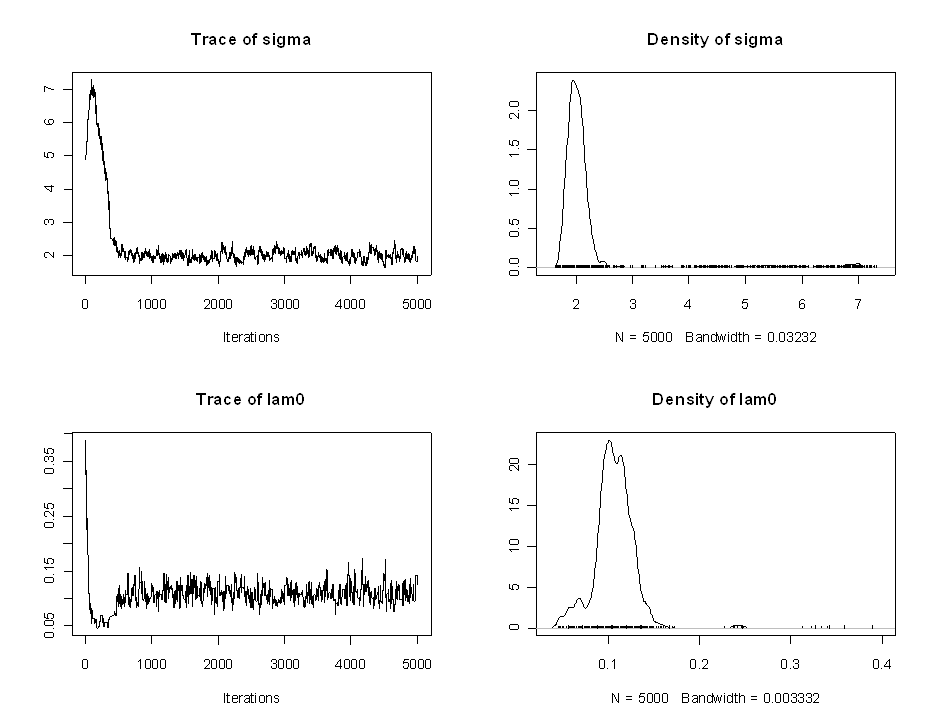
\includegraphics[height=2.5in]{Ch6/figs/timeseries}
\end{center}
\caption{Time series and posterior density plots for $\sigma$ and $\lambda_0$.}
\label{timeseries.fig}
\end{figure}


Second, you will be able to see if your chains converged and how many initial simulations you have to discard as burn-in. In the case of the chains shown in Fig. \ref{timeseries.fig}, we would probably consider the first 750 - 1000 iterations as burn-in, as afterwards the chains seem to be fairly stationary.

\subsection{Posterior density plots}
The \verb#plot()# command also produces posterior density plots and it is worthwhile to look at those carefully. For parameters with priors that have bounds (e.g. Uniform over some interval), you will be able to see if your choice of the prior is truncating the posterior distribution. In the context of SCR models, this will mostly involve our choice of $M$, the size of the augmented data set. If the posterior of $N$ has a lot of mass concentrated close to $M$ (or equivalently the posterior of $\psi$ has a lot of mass concentrated close to 1), as in the example in Fig. \ref{timeseries2.fig}, we have to re-run the analysis with a larger $M$.  A flat posterior plot shows you that the parameter essentially cannot be identified. There may not be enough information in your data to estimate model parameters and you may have to consider a simpler model. Finally, posterior density plots will show you if the posterior distribution is symmetrical or skewed -- if the distribution has a heavy tail, using the mean as a point estimate of your parameter of interest may be biased and you may want to opt for the median or mode instead.

\begin{figure}
\begin{center}
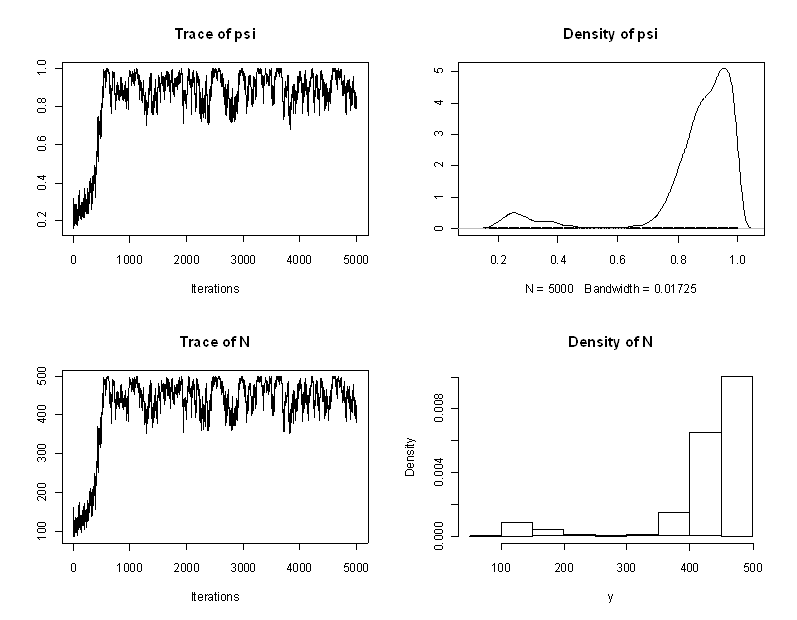
\includegraphics[height=2.5in]{Ch6/figs/timeseries2}
\end{center}
\caption{Time series and posterior density plots of $\psi$ and $N$ for the bear data set truncated by the upper limit of $M$ (500).}
\label{timeseries2.fig}
\end{figure}

\subsection{Serial autocorrelation and effective sample size}
Checking the degree of autocorrelation in your Markov chains and estimating the effective sample size your chain has generated should be part of evaluating your model output. If you use WinBUGS through the R2WinBUGS package, the \verb#print()# command will automatically return the effective sample size for all monitored parameters. In the coda package there are several functions you can use to do so. \verb#effectiveSize()# will directly give you an estimate of the effective sample size for you parameters:
\begin{verbatim}
> effectiveSize(chain)
    sigma      lam0       psi         N
 3.930303 78.259159 30.436348 32.047392
\end{verbatim}

Alternatively, you can use the \verb#autocorr.diag()# function, which will show you the degree of autocorrelation for different lag values (which you can specify within the function call, we use the defaults below):
\begin{verbatim}
> autocorr.diag(mcmc(mod))
           sigma      lam0       psi         N
Lag 0  1.0000000 1.0000000 1.0000000 1.0000000
Lag 1  0.9979948 0.9494134 0.9847503 0.9774201
Lag 5  0.9915567 0.8038168 0.9111951 0.9113525
Lag 10 0.9836016 0.6714021 0.8462108 0.8509803
Lag 50 0.8985337 0.1983780 0.6138516 0.6233994
\end{verbatim}
In the present case we see that autocorrelation is especially high for the parameter $\sigma$ and our effective sample size for this parameter is 4! \footnote{Anyone have any idea how the autocorrelation in sigma could be reduced?} This means we would have to run the model for much longer to obtain a reasonable effective sample size. Unfortunately, with many SCR models we observe high degrees of serial autocorrelation. For now, let's continue using this small set of samples to continue looking at the output.


\subsection{Summary results}
Now that we checked that our chains apparently have converged and pretending that we have generated enough samples from the posterior distribution, we can look at the actual parameter estimates. The \verb#summary()# function will return two sets of results: the mean parameter estimates, with their standard deviation, the naïve standard error -- i.e. your regular standard error calculated for $T$ (= number of iterations) samples without accounting for serial autocorrelation -- and the Time-series SE (in WinBUGS and earlier in this book referred to as MC error), which accounts for autocorrelation. Remember our rule of thumb that this error decreases with increasing chain length and should be 1\% or less of the parameter estimate.In WinBUGS the MC error is only given in the log output within BUGS itself.
You should adjust the \verb#summary()# call by removing the burn-in from
calculating parameter summary statistics. To do so, use the \verb#window()#
command, which lets you specify at which iteration to start
'counting'. In contrast to WinBUGS, which requires you to set the
burn-in length before you run the model, this command gives us full
flexibility to make decisions about the burn-in after we have seen the
trajectories of our Markov chains. For our example,
\verb#summary(window(chain, start=1001))# returns the following output:


\begin{verbatim}
Iterations = 1001:5000
Thinning interval = 1
Number of chains = 1
Sample size per chain = 4000

1. Empirical mean and standard deviation for each variable,
   plus standard error of the mean:

          Mean       SD  Naive SE Time-series SE
sigma   1.9986  0.13805 0.0021827       0.016091
lam0    0.1096  0.01523 0.0002407       0.001401
psi     0.6113  0.09148 0.0014465       0.010734
N     489.8535 71.79695 1.1352094       8.431119

2. Quantiles for each variable:

           2.5%       25%      50%      75%    97.5%
sigma   1.75780   1.89847   1.9900   2.0944   2.2772
lam0    0.08357   0.09824   0.1087   0.1192   0.1427
psi     0.45110   0.54838   0.6052   0.6639   0.8192
N     366.00000 440.00000 485.0000 530.0000 654.0000
\end{verbatim}

Looking at the MC errors, we see that in spite of the high autocorrelation, the MC error for $\sigma$ is below the 1\% threshold, whereas for all other parameters, MC errors are still above, another indication that for a thorough analysis we should run a longer chain.
Our algorithm gives us a posterior distribution of $N$, but we are usually interested in the density, $D$. Density itself is not a parameter of our model, but we can derive a posterior distribution for $D$ by dividing each value of $N$ ($N$ at each iteration) by the area of the state-space (here 3032.719 km$^2$) and we can use summary statistics of the resulting distribution to characterize $D$:
\begin{verbatim}
> summary(window(chain[,4]/ 3032.719, start=1001))
Iterations = 1001:5000
Thinning interval = 1
Number of chains = 1
Sample size per chain = 4000

1. Empirical mean and standard deviation for each variable,
   plus standard error of the mean:

          Mean             SD       Naive SE Time-series SE
     0.1615229      0.0236741      0.0003743      0.0027801

2. Quantiles for each variable:

  2.5%    25%    50%    75%  97.5%
0.1207 0.1451 0.1599 0.1748 0.2156
\end{verbatim}
We see that our mean density of $0.16/km^2$ is very similar to the estimate of $0.18/km^2$ obtained under the non-spatial model M0 in Chapt. \ref{chapt.closed}.


\subsection{Other useful commands }
While inspecting the time series plot gives you a first idea of how well you tuned your MH algorithm, use \verb#rejectionRate()# to obtain the rejection rates (1 -- acceptance rates) of the parameters that are written to your output:
\begin{verbatim}
> rejectionRate(chain)
     sigma       lam0        psi          N
0.44108822 0.77675535 0.00000000 0.01940388
\end{verbatim}
 Recall that rejection rates should lie between 0.2 and 0.8, so our tuning seems to have been appropriate here. $\psi$ is never rejected since we update it with Gibbs sampling, where all candidate values are kept. And since $N$ is the sum of all $z_i$, all it takes for $N$ to change from one iteration to the next are small changes in the z-vector, so the rejection rate of $N$ is always low.
If you have run several parallel chains, you can combine them into a single mcmc object using the \verb#mcmc.list()# command on the individual chains (note that each chain has to be converted to an mcmc object before combining them with \verb#mcmc.list()#). You can then easily obtain the Gelman-Rubin diagnostic \citep{gelman_etal:2004}, in WinBUGS called R-hat, using \verb#gelman.diag()#, which will indicate if all chains have converged to the same stationary distribution.
For details on these and other functions, see the coda manual, which can be found (together with the package) on the CRAN mirror.

\section{Manipulating the state-space}
So far, we have constrained the location of the activity centers to fall within the outermost coordinates of our rectangular state space by posing upper and lower bounds for $x$ and $y$. But what if $S$ has an irregular shape -- maybe there is a large water body we would like to remove from $S$, because we know our terrestrial study species does not occur there. Or the study takes place in a clearly defined area such as an island. As mentioned before, this situation is difficult to handle in WinBUGS. In some simple cases we can adjust the state space by setting $s_{xi}$ to be some function of $s_{yi}$ or vice versa. In this manner, we can cut off corners of the rectangle to approximate the actual state space. In R, we are much more flexible, as we can use the actual state-space polygon to constrain out $s_i$. \footnote{ Have to check if we can use panther stuff for the book; otherwise, use raccoon example.}To illustrate that, let's look at a camera trapping study of Florida panthers (\emph{Puma concolor coryi}) conducted in the Picayune Strand Restoration Project (PSRP) area, southwest Florida (Fig. \ref{pantercamera.fig}), by XXX, and financed by XXX. In the 1960ies the PSRP area was slated for housing development, but then bought back by the State of Florida and is currently being restored to its original hydrology and vegetation. In an effort to estimate the density of the local Florida panther population, 98 camera traps were operated in the area for 21 months between 2005 and 2007. Florida panthers are wide-ranging animals and in order to account for their wide movements, the state-space was defined as the trapping grid buffered by 15 km around its outermost coordinates. However, the resulting rectangle contained some ocean in its southwestern corner (Fig. \ref{pantercamera.fig}).
In order to precisely describe the state-space, the ocean has to be removed. You can create a precise state-space polygon in ArcGIS and read it into R, or create the polygon directly within R. In the present case we intersected two shape files -- one of the state of Florida and one of the rectangle defined by a strip of 15 km around the camera-trapping grid.
While you will most likely have to obtain the shapefile describing the landscape of and around your trapping grid (coastlines, water bodies etc.) from some external source, a polygon shapefile buffering your outermost trapping grid coordinates can easily be written in R.

If xmin, xmax, ymin and ymax, mark the outermost $x$ and $y$ coordinates of your trapping grid and $b$ is the distance you want to buffer with, load the package shapefiles \citep{stabler:2006} and use:
\begin{verbatim}
xl= xmin-b
xu= xmax+b
yl= ymin-b
yu= ymax+b

dd <- data.frame(Id=c(1,1,1,1,1),X=c(xl,xu,xu,xl,xl),Y=c(yl,yl,yu,yu,yl)) #create data frame with coordinate pairs
ddTable <- data.frame(Id=c(1),Name=c("Item1"))
ddShapefile <- convert.to.shapefile(dd, ddTable, "Id", 5) #convert #to shapefile, type polygon
write.shapefile(ddShapefile, 'c:/…’, arcgis=T) # save to location of #choice
\end{verbatim}


\begin{figure}
\begin{center}
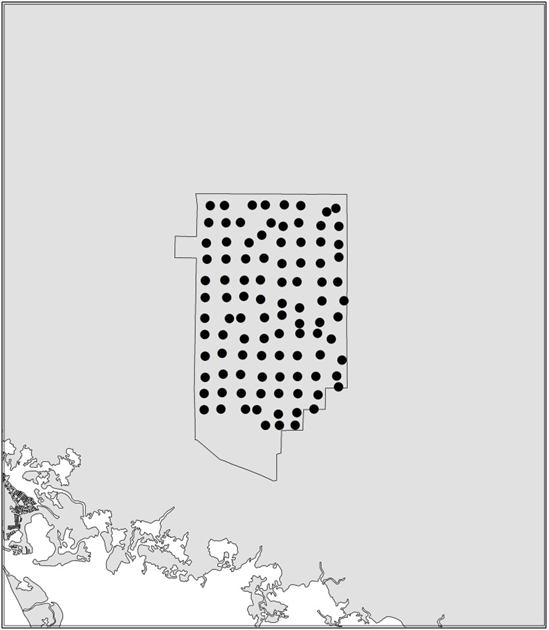
\includegraphics[height=2.5in]{Ch6/figs/panthercamera}
\end{center}
\caption{Rectangular state-space for a Florida panther camera trapping
study in the PSRP area (grey outline, red block inset map of Florida)
contain some ocean (white) that needs to be removed from the state-space.}
\label{pantercamera.fig}
\end{figure}

You can read shapefiles into R loading the package maptools
\citep{lewin-koh_etal:2011} and using the function
\verb#readShapeSpatial()#. Make sure you read in shapefiles in UTM format, so
that units of the trap array, the movement parameter sigma and the
state-space are all identical.  Intersection of polygons can be done
in R also, using the package rgeos \citep{bivand_rundel:2011} and the
function \verb#gIntersect()#. The area of your (single) polygon can be
extracted directly from the state-space object SSp:

\begin{verbatim}
> area <- SSp@polygons[[1]]@Polygons[[1]]@area /1000000
\end{verbatim}

 Note that dividing by 1000000 will return the area in km$^2$ if your coordinates describing the polygon are in UTM. If your state-space consists of several disjunct polygons, you will have to sum the areas of all polygons to obtain the size of the state-space.
To include this polygon into our MCMC sampler we need one last spatial R package, sp \citep{pebesma_bivand:2011}, which has a function, \verb#over()#, which allows us to check if a pair of coordinates falls within a polygon or not. All we have to do is embed this new check into the updating steps for $s$:
\begin{verbatim}
        Scand <- as.matrix(cbind(rnorm(M, S[,1], 2),
                   rnorm(M, S[,2], 2)))	        #draw candidate value

	Scoord<-SpatialPoints(Scand*1000)    #convert to spatial points on UTM (m) scale
	SinPoly<-over(Scoord,SSp)		# check if scand is within the polygon

       for(i in 1:M) {
	if(is.na(SinPoly[i])==FALSE) {		#if scand falls within polygon, continue update
… [rest of the updating step remains the same]
\end{verbatim}
Note that it is much more time-efficient to draw all $M$ candidate values for $s$ and check once if they fall within the state-space, rather than running the \verb#over()# command for every individual pair of coordinates. To make sure that our initial values for s also fall within the polygon of $S$, we use the function \verb#runifpoint()# from the package spatstat \citep{baddeley_turner:2005}, which generates random uniform points within a specified polygon. You'll find this modified MCMC algorithm (SCR0poisSSp) in the R packe scrbook.
Finally, observe that we are converting candidate coordinates of $S$ back to meters to match the UTM polygon. In all previous examples, for both the trap locations and the activity centers we have used UTM coordinates divided by 1000 to estimate $\sigma$ on a km scale. This is adequate for wide ranging individuals like bears. In other cases you may center all coordinates on 0. No matter what kind of transformation you use on your coordinates , make sure to always convert candidate values for $S$ back to the original scale (UTM) before running the \verb#over()# command.

\section{MCMC software packages}
Throughout most of this book we will use WinBUGS and, occasionally, JAGS to run MCMC analyses. Here, we will briefly discuss the main pros and cons of these two programs as well as WinBUGS successor OpenBUGS. 

\subsection{WinBUGS}
In a nutshell, WinBUGS (and the other programs) do everything that we just went through in this chapter (and quite a bit more). Looking through your model, WinBUGS determines which parameters it can use standard Gibbs sampling for (i.e. for conjugate full conditional distributions). Then, it determines, in the following hierarchy, whether to use adaptive rejection sampling, slice sampling or -- in the 'worst' case -- Metropolis-Hastings sampling for the other full conditionals \citep{spiegelhalter_etal:2003}. If it uses MH sampling, it will automatically tune the updater so that it works efficiently.
While WinBUGS is a convenient piece of software that is still widely used, its major drawback is that it is no longer being developed, i.e. no new functions or distributions are added and no bugs are fixed.

\subsection{OpenBUGS}
OpenBUGS is essentially the successor of WinBUGS. While the latter is
no longer worked on, OpenBUGS is constantly developed further. The
name 'OpenBUGS' refers to the software being open source, so users do
not need to download a license key, like they have to for WinBUGS
(although the license key for WinBUGS is free and valid for life).

Compared to WinBUGS, OpenBUGS has a lot more built-in functions. The
method of how to determine the right updater for each model parameter
has changed and the user can manually control the MCMC algorithm used
to update model parameters.  Several other changes have been
implemented in OpenBUGS and a detailed list of differences between the
two BUGS versions, can be found at
http://www.openbugs.info/w/OpenVsWin

While OpenBUGS is a useful program for a lot of MCMC sampling
applications, for reasons we do not understand, simple SCR models do
not converge in OpenBUGS. It is therefore advisable that you check any
OpenBUGS SCR model results against result from WinBUGS. Also,
currently, the R package BRugs \citep{thomas_etal:2006}, necessary
for running OpenBUGS through R, has problems with 64-bit machines, so
you may have to use the 32-bit version of R and OpenBUGS in order to
make it work. The BUGS project site at http://www.openbugs.info
provides a lot of information on and download links for OpenBUGS.

There is an extensive help archive for both WinBUGS and OpenBUGS and you can subscribe to a mailing list, where people pose and answer questions of how to use these programs at http://www.mrc-bsu.cam.ac.uk/bugs/overview/list.shtml

\subsection{JAGS -- Just Another Gibbs Sampler}
JAGS, currently at Version 3.1.0, is another free program for analysis of Bayesian hierarchical models using MCMC simulation. Originally, JAGS was the only program using the BUGS language that would run on operating systems other than the 32 bit Windows platforms. By now, there are OpenBUGS versions for Linux or Macintosh machines.
JAGS 'only' generates samples from the posterior distribution; analysis of the output is done in R, either by running JAGS through R using either the packages rjags \citep{plummer:2011} or R2jags \citep{su_yajima:2011}, or by using coda on your JAGS output. The program, manuals and rjags can be downloaded at http://sourceforge.net/projects/mcmc-jags/files/
When run from within R using the package rjags or R2jags, writing a JAGS model is virtually identical to writing a WinBUGS model. However, some functions may have slightly different names and you can look up available functions and their use in the JAGS manual. One potential downside is that JAGS can be very particular when it comes to initial values. These may have to be set as close to truth as possible for the model to start. Although JAGS lets you run several parallel Markov chains, this characteristic interferes with the idea of using overdispersed initial values for the different chains. Also, we have occasionally experienced JAGS to crash and take the R GUI with it. Only re-installing both JAGS and rjags seemed to solve this problem.
On the plus side, JAGS usually runs a little faster than WinBUGS, sometimes considerably faster (see Sect. \ref {4.XYZ}), is constantly being developed and improved and it has a variety of functions that are not available in WinBUGS. For example, JAGS allows you to supply observed data for some deterministic functions of unobserved variables. In BUGS we cannot supply data to logical nodes. Another useful feature is that the adaptive phase of the model (the burn-in) is run separately from the sampling from the stationary Markov chains. This allows you to easily add more iterations to the adaptive phase if necessary without the need to start from 0. There are other, more subtle differences and there is an entire manual section on differences between JAGS and OpenBUGS.
For questions and problems there is a JAGS forum online at http://sourceforge.net/projects/mcmc-jags/forums/forum/610037.
\footnote{As we make progress on the book, lets be sure  to add linkages to places where we use JAGS in examples.}

\section{Summary and Outlook}
While there are a number of flexible and extremely useful software packages to perform MCMC simulations, it sometimes is more efficient to develop your own MCMC algorithm. Building an MCMC code follows three basic steps: Identify your model including priors and express full conditional distributions for each model parameter. If full conditionals are parametric distributions, use Gibbs sampling to draw candidate parameter values from this distributions; otherwise use Metropolis-Hastings sampling to draw candidate values from a proposal distribution and accept or reject them based on their posterior probability densities.
These custom-made MCMC algorithms give you more modeling flexibility than existing software packages, especially when it comes to handling the state-space: In BUGS (and JAGS for that matter) we define a continuous rectangular state-space using the corner coordinates to constrain the Uniform priors on the activity centers $s$. But what if a continuous rectangle isn't an adequate description of the state-space? In this chapter we saw that in R it only takes a few lines of code to use any arbitrary polygon shapefile as the state-space, which is especially useful when you are dealing with coastlines or large bodies of water that need removing from the state-space. Another example is the SCR R package SPACECAP \citep{gopalaswamy_etal:2011} that was developed because implementation of an SCR model with a discrete state-space was inefficient in WinBUGS.
Another situations in which using BUGS/JAGS becomes increasingly complicated or inefficient is when using point processes other than the Uniform Poisson point process which underlies the basic SCR model (see Chapt. \ref {Chapter X}). In the Chapt. \ref {Chapter X} and XX you will see examples of different point processes, implemented using custom-made MCMC algorithms. \footnote{Richard, Beth expand on that?}
Finally, the Chapt. \ref {Chapter X} and XX deal with unmarked or partially marked populations using hand-made MCMC algorithms to handle the (partially) latent individual encounter histories. While some of these models can be written in BUGS/JAGS, \footnote{the Poisson one for partially marked we wrote in BUGS and it should work with a known number of marked; the Bernoulli in JAGS with the dsum() function should work for the fully unknown; maybe some others? I don’t remember. We may have to try writing the others before saying that they don’t work in BUGS/JAGS; they are certainly much faster in R, though.}, they are painstakingly slow; others cannot be implemented in BUGS/JAGS at all.
In conclusion, while you can certainly get by using BUGS/JAGS for standard SCR models, knowing how to write your own MCMC sampler allows you to tailor these models to your specific needs.
